\documentclass{article}
\usepackage{graphicx} % Required for inserting images
\usepackage{amsmath}
\usepackage{esvect}
\usepackage{booktabs}
\usepackage{float}
\usepackage{enumerate}
\usepackage{hyperref}

\title{\textbf{Secure Multi-Party Computation
}Assignment 1 - Truth-table and circuits for sign activation\textbf{}}
\author{Or Dinar \\
Liad Ackerman}
\date{06.01.2024}

\begin{document}

\maketitle

\paragraph{\LARGE Exercise 1\\\\}

Write the Truth-table for the function specified in Equation 2. The Truth-table specifies the function values for all possible assignments to $\overrightarrow{a},\overrightarrow{x}\in \left\{ 0,1,2,3\right\}$

\paragraph{Equation 2:}

$$
f_{a,4}(x)=\begin{cases}
			1 & \text{if $ax \geq 4$ }\\
            0 & \text{otherwise}
		 \end{cases} \hspace{1cm} for \hspace{.25cm}a\in \left\{ 0,1,2,3\right\}
$$
\\
The Truth-table for given equation will look like the following table:

\begin{figure}[H]
    \centering
    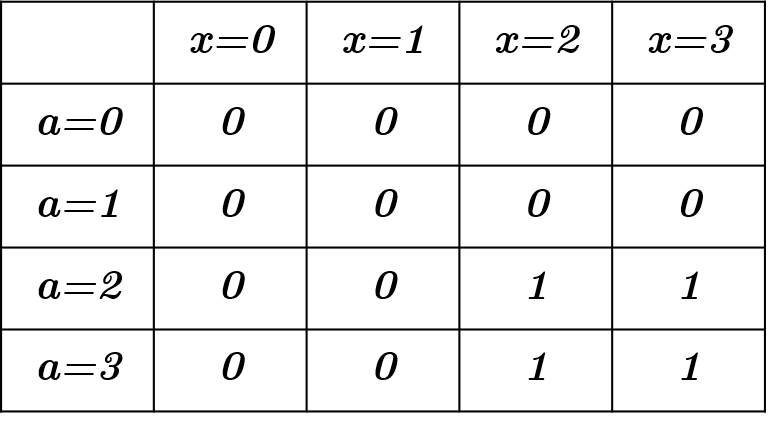
\includegraphics[width=0.5\linewidth]{Picture1.png}
    \caption{Truth-table for equation 2.}
    \label{fig:enter-label}
\end{figure}
\newpage 
\paragraph{\LARGE Exercise 2\\\\}

Write a Boolean circuit computing the function specified in Equation 3, with XOR
and AND gates.

\paragraph{Equation 3:}

$$
f_{\overrightarrow{a},4}(x_{1},x_{2})=\begin{cases}
			1 & \text{if $a_1x_1 + a_2x_2 \geq 4$ }\\
            0 & \text{otherwise}
		 \end{cases} \hspace{1cm} for \hspace{.25cm}  \overrightarrow{a} \in {\left\{ 0,1,2,3\right\}}^{2}
$$
\\
In order to construct a Boolean circuit that represents $equation$ $3$, we first need to construct Boolean circuits for multiplying 2-bit numbers, and for adding of 4-bit numbers.


\begin{figure}[H]
    \centering
    
\includegraphics[width=1\linewidth]{1920px-Binary_multiplier.svg.png}
    \caption
    {
    A multiplication Boolean circuit for multiplying 2-bit numbers, as seen in \textit{Binary Multiplier - Wikipedia}$^{1}$.
    }
    \label{fig:enter-label}
\end{figure}


The product of 2-bit numbers $A$ and $B$, whereas A$_0$, A$_1$ and B$_0$, B$_1$ are the bits of A and B respectively, Is the number C whereas C$_0$, C$_1$, C$_2$, C$_3$ are the bits of C.
\\
We will refer to the Boolean circuit from Figure 2 as 2-bit MULTI.
\\\\
In order to make an addition Boolean circuit for two 4-bit numbers we will have to use OR gates. Since we can not use OR gates we will represent them using only AND and XOR gates. We'll use the Truth-tables of AND and XOR to infer how the wanted Boolean circuit will look like. 

\begin{figure}[H]
    \centering
    
\includegraphics[width=1\linewidth]{Picture2.png}
    \caption{Truth-tables for XOR and AND gates.}
    \label{fig:enter-label}
\end{figure}

\begin{figure}[H]
    \centering
    
\includegraphics[width=0.4\linewidth]{Picture3.png}
    \caption{Truth-table for OR gates.}
    \label{fig:enter-label}
\end{figure}

The following Boolean circuit has the same Truth-table as an OR gate:
\begin{figure}[H]
    \centering
    
\includegraphics[width=1\linewidth]{OR GATE.png}
    \caption{OR gate represented by AND and XOR gates only}
    \label{fig:enter-label}
\end{figure}
Now that we can use OR gates we can create an addition boolean circuit that will be referred to as 4-bit ADDER. See below:

\begin{figure}[H]
    \centering
    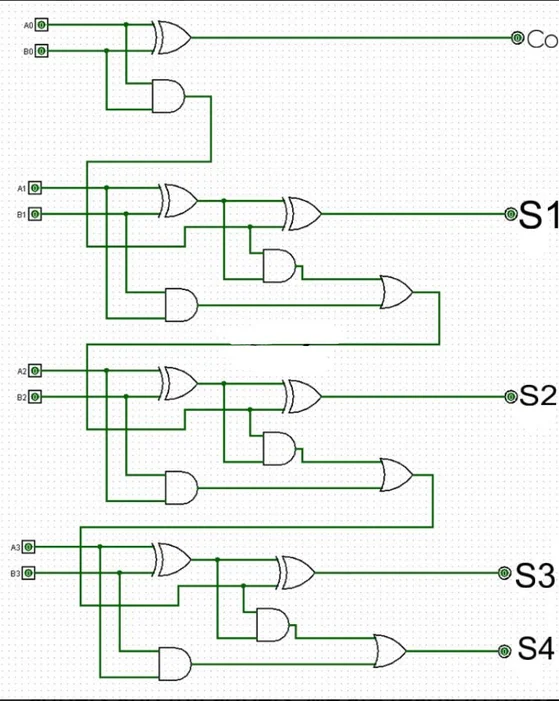
\includegraphics[width=1\linewidth]{FMUD6P1LJ1FVETK.png}
    \caption{Addition boolean circuit as seen in $instructables.com$ $-$ $4$ $Bit$ $Binary$ $Adder$ $^2$.}
    \label{fig:enter-label}
\end{figure}
\newpage
\paragraph {Observation:} a binary number is greater or equal than 4 (in decimal) when either the 3rd or 4th bits are 1, meaning we will take the product of all calculations and run the 3rd, 4th and the carry out bit through an OR gate, that will guarantee us the product is greater or equal to 4.



The final Boolean circuit will be the following:
\\
\begin{figure}[H]
    \centering
    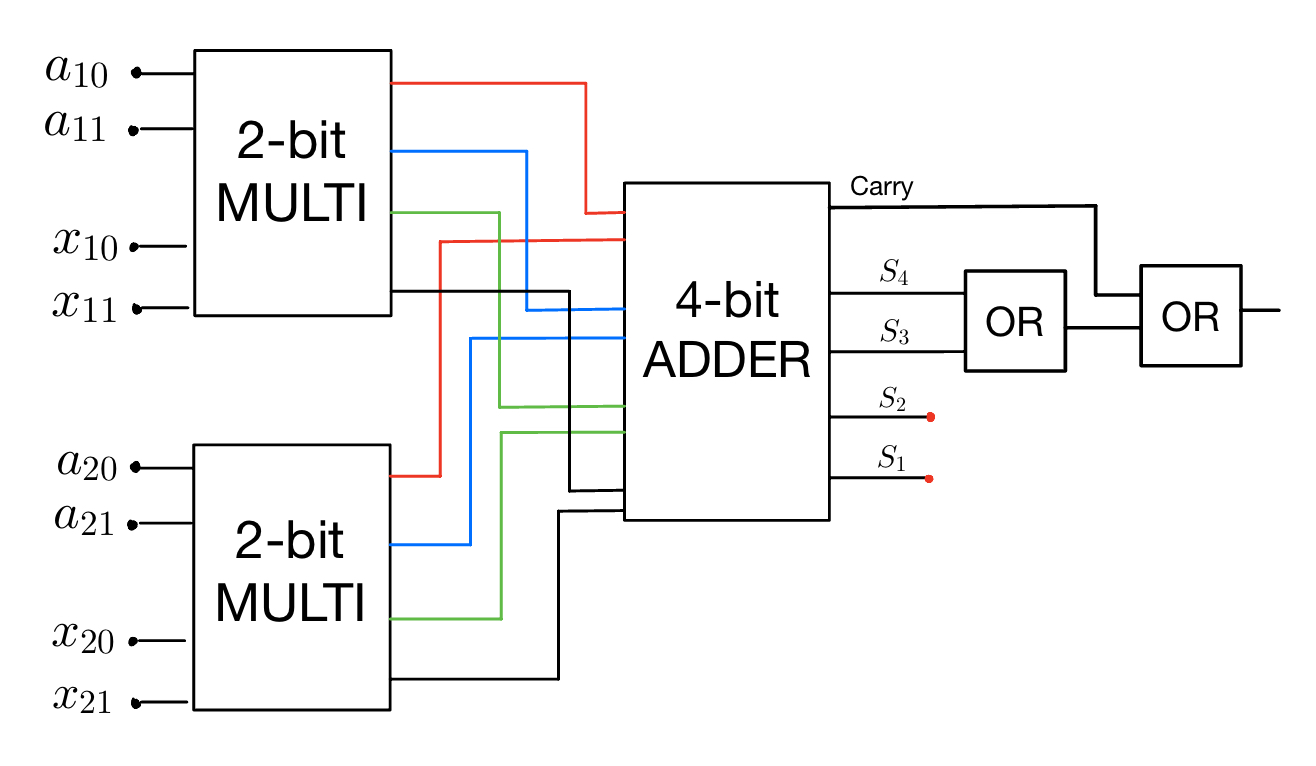
\includegraphics[width=1\linewidth]{FinalBooleanCircuit.jpeg}
    \caption{Boolean circuit that represents $Equation$ $3$.}
    \label{fig:enter-label}
\end{figure}

\newpage
\paragraph{\LARGE Exercise 3\\\\}
In this exercise we are being asked to create an arithmetic circuit under the field $GF(11)$, where we have addition and multiplication gates $mod$ $11$. Equation is still equation (3):
\paragraph{Equation 3:}

$$
f_{\overrightarrow{a},4}(x_{1},x_{2})=\begin{cases}
			1 & \text{if $a_1x_1 + a_2x_2 \geq 4$ }\\
            0 & \text{otherwise}
		 \end{cases} \hspace{1cm} for \hspace{.25cm}  \overrightarrow{a} \in {\left\{ 0,1,2,3\right\}}^{2}
$$
\paragraph{Note:} The gates in the circuit are closed under the field GF(11), which means and addition gate is $mod$ $11$ and so is the multiplication gate.
\\In the circuit, first, we add the multiplications of $a_1x_1$ and $a_2x_2$ like so:
\begin{figure}[H]
    \centering
    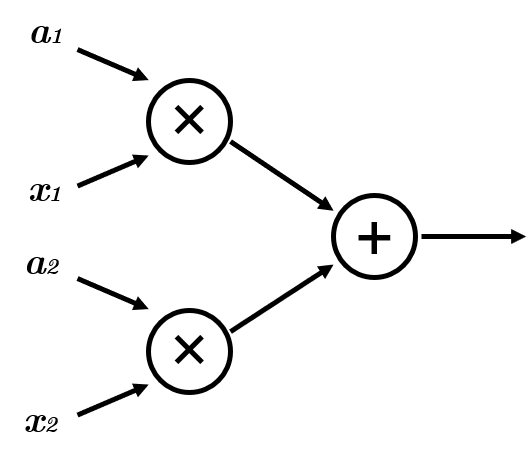
\includegraphics[width=.5\linewidth]{arithcirc.png}
    \caption{Adding the product of $a_1x_1$ and $a_2x_2$}
    \label{fig:enter-label}
\end{figure}

Now we have a value that we can compare to $4$ ($mod$ $11$), we will denote it as $SUM$. After discussing the issue with Dr. Akavia we reached the conclusion that we can use Fermat's little theorem in order to compare both sides of the equation. The claim of the theorem is the following:

$$
a^{p-1}  \equiv\begin{cases}
			0 \hspace{.25cm} (mod \hspace{.25cm}p) & \text{if $a = 0$}\\
            1 \hspace{.25cm} (mod \hspace{.25cm}p) & \text{otherwise}
		 \end{cases} \hspace{1cm} for \hspace{.1cm}  p \hspace{.1cm}is \hspace{.1cm}prime
$$

Furthermore, we can say that for every $k \in GF(11)$:
\\
$(SUM-k)^{10} \equiv 0 \hspace{.25cm} (mod \hspace{.25cm} 11)$
if and only if SUM = k. That means we can implement an arithmetic circuit to compare two numbers in a field, therefore we can compare SUM to each of the values in $\left\{ 4,5,6,7,8,9,10\right\}$. 
\\Note that $-k$ $\equiv$ $11-k$ ($mod$ $11$). That means that instead of preforming $(SUM + (-k))$ $for$ $k$ $\in \left\{ 4,5,6,7,8,9,10\right\}$, we can preform $(SUM + k)$\\ $for$ $k$ $\in \left\{ 7,6,5,4,3,2,1\right\}$. The implementation of such circuit is the following:

\begin{figure}[H]
    \centering
    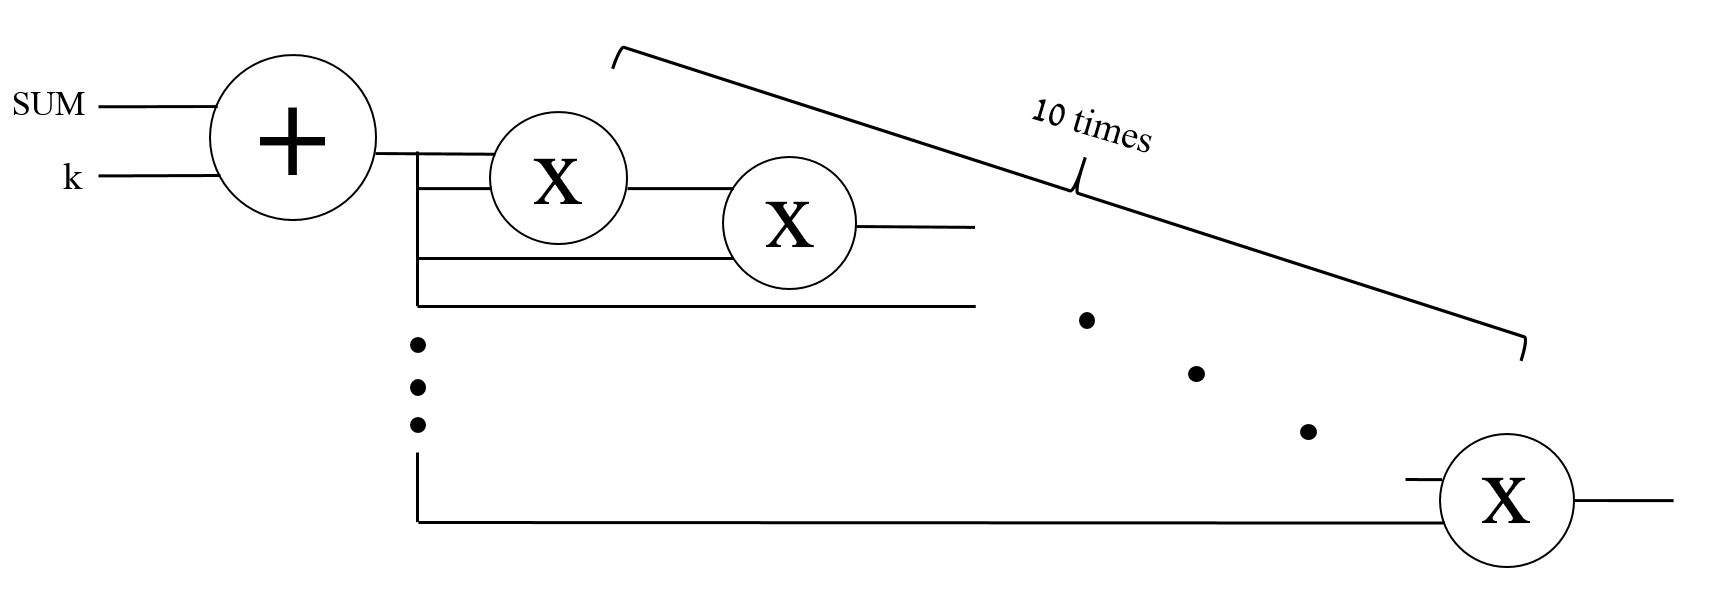
\includegraphics[width=1\linewidth]{comparisonGate.png}
    \caption{Implementation of $(SUM+k)^{10}$. It returns 0 if $SUM=k$,\\ and 1 otherwise.}
    \label{fig:enter-label}
\end{figure}

Now, we can implement this operation seven times, one for each $k$ $\in \left\{ 7,6,5,4,3,2,1\right\}$. As said before - the calculation in Figure 9 returns 0 if $SUM=k$, and 1 otherwise. which means that after adding the return value of each of the seven operations (we will refer it as $TOTAL$), we should get $TOTAL=7$ if $SUM \neq -k$ for every $k$ $\in \left\{ 7,6,5,4,3,2,1\right\}$ and 6 otherwise (Because there can be at most one equality). The above can be written as the equation:

$$
TOTAL  \equiv\begin{cases}
			7 & \text{if $SUM < 4$}\\
            6  & \text{$SUM \geq  4$}
		 \end{cases} 
$$
Which brings us closer to the solution. We would like to map $7\mapsto 0$ and $6\mapsto 1$. One way we can do that, is by adding 5 to TOTAL (which maps $7\mapsto 0$ and $6\mapsto 10$) and using Fermat's little theorem again to conclude that:
$$
a^{10}  \equiv\begin{cases}
			0 \hspace{.25cm} (mod \hspace{.25cm}11) & \text{if $a = 0$}\\
            1 \hspace{.25cm} (mod \hspace{.25cm}11) & \text{if $a = 10$}
		 \end{cases}
$$

In conclusion - we need to return $(TOTAL+5)^{10}$. The implementation of such circuit is the following:

\begin{figure}[H]
    \centering
    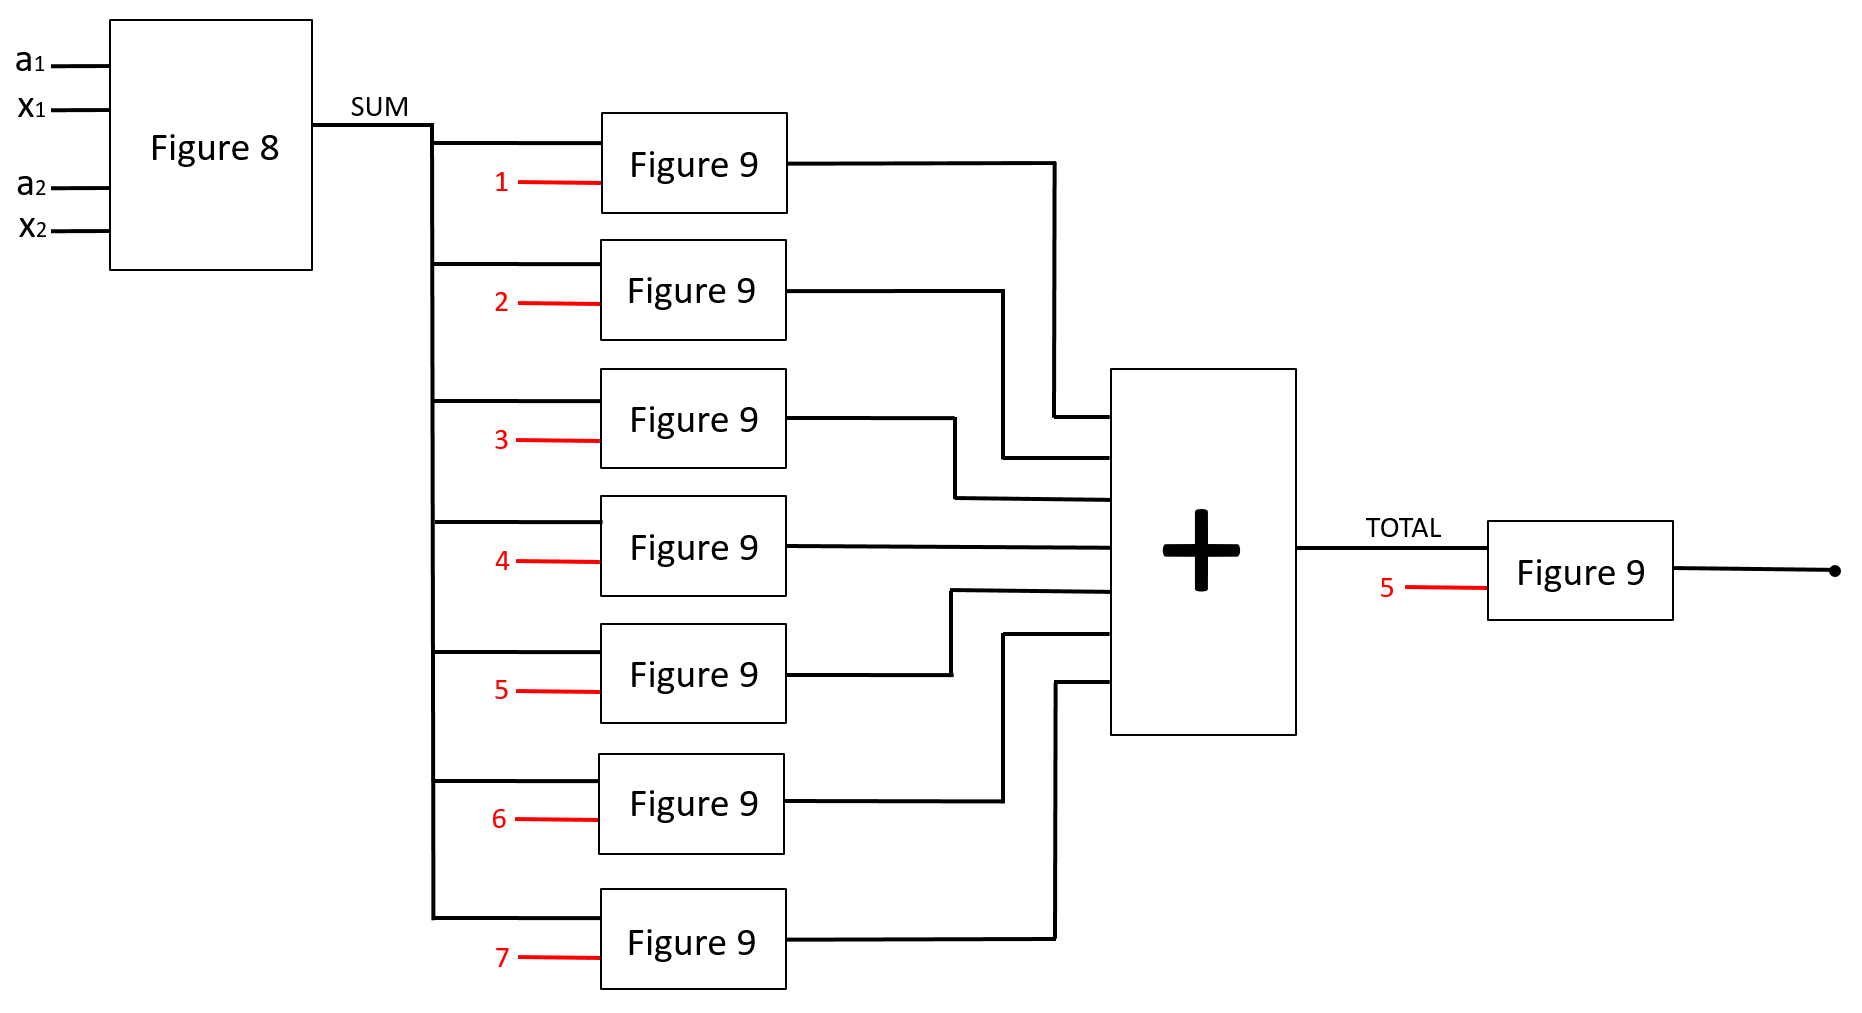
\includegraphics[width=1.25\linewidth]{FinalArithmeticCircuit.png}
    \caption{Arithmetic circuit that represents $Equation$ $3$.}
    \label{fig:enter-label}
\end{figure}


\newpage
\paragraph{\LARGE Exercise 4\\\\}

\begin{enumerate}[i]
  \item Circuit Depth\
  The maximal length of an input is the largest path an input can traverse the circuit in order to get to the end of it, technically all paths are the same so we will calculate the path from the input to the output.
  The depth of Figure 8 is 3. The depth of figure 9 is 11, and it appears twice in a path. Therefore the depth is $3+11+1+11=$\textbf{26 gates}.
  \item Circuit Size\
  We will sum the total amount of gates in the circuit to conclude the size, in figure 9 we have 10 multiplication gates and one addition gate, The figure appears 8 times. in figure 8 we have 3 gates. And we also have the  addition gate at the end.\
  All in all we have $ 11\times 8 + 3 + 1 =$ \textbf{92 gates}.
  \item x-depth\
  The multiplicative depth is the amount of multiplications in a maximal path. The amount of multiplications in Figure 8 is 1, and the amount of multiplications in Figure 9 is 10, therefore the x-depth is $1+10+10=$ \textbf{21 gates}.
  \item \# MULT\
  The amount of multiplication gates in the arithmetic circuit, since there are 8 Figure 9's (10 multiplication gates in each), and one Figure 8 (2 multiplication gates), the amount of multiplication gates is $10\times8+1\times2=$ \textbf{82 multiplication gates}.
\end{enumerate}

\newpage

\section{Bibliography}
$^{1}$ - \url{https://en.wikipedia.org/wiki/Binary_multiplier} - Binary multiplier - Wikipedia.\\
$^{2}$ - \url{https://www.instructables.com/4-Bit-Binary-Adder-FINAL-PROJECT/} - 4 Bit Binary Adder.\\
$^{3}$ - Dr. Akavia's proposal for using Fermat's little Theorem.

\end{document}
